\documentclass[]{article}
\usepackage[czech]{babel}
\usepackage[utf8]{inputenc}
\usepackage{float}
\usepackage{graphicx}


\begin{document}

\title{Kapitola 1: Definice základních pojmů}
\author{Bc. Štěpán Heller}
\date{\today}
\maketitle

\section{Motivace k řízení podnikových procesů}
Každá firma, která se snaží efektivně řídit svůj chod a neustále se rozvíjet stále hledá nové a nové cesty, jak toho docílit. Takovými cestami může být uvádění nových produktů na trh, hledání nových trhů a příležitostí na nich, nabírání nových zaměstnanců, investice do propracovaného marketingu a mnoho dalších. Stále více firem ale v posledních několika dekádách obrací svou pozornost také dovnitř vlastní organizace. Hledají oblasti, kde je možné najít úspory nebo kde by bylo možné práci zefektivnit.

Aby bylo něco takového vůbec možné, musí mít manažeři a odpovědní vedoucí pracovníci především přehled o své organizaci a její hlubokou znalost. Pouze z takové hluboké znalosti pak mohou vzejít příležitosti k efektivnějšímu dosahování podnikových cílů.

Z toho důvodu firmy a organizace hledají cesty, jak lépe pochopit a následně standardizovat \textit{procesy} v rámci vlastního podniku, které ve svém souhrnu nejsou nic jiného než soubor postupů, kterými podnik nebo organizace dosahuje svých cílů. O tom, kterak takové procesy pozorovat, standardizovat a řídit, byla napsána celá řada publikací a je nezbytné mít na zřeteli, že se jednotlivé přístupy od sebe více či méně odlišují. 

Ačkoliv akademici i odpovědní lidé z prostředí samotných firem a organizací se často přou, který z přístupů je lepší, zůstává bez nejmenších pochyb, že adoptování jakéhokoliv přístupu vedoucího k lepšímu porozumění chodu vlastní organizace je lepší, než nahodilý přístup k řízení společnosti, kdy jsou změny vykonávany ad hoc a jakékoliv plánování do budoucna je tak velmi obtížné. Pochopení vlastní organizace je jedním (nikoli jediným) ze základních předpokladů pro její dlouhodbě udržitelný rozvoj a právě k tomu jsou procesy a procesní řízení široce akceptovaným přístupem.

The main objective of process management is to find the most efficient and effective way to transform customer requirements into customer satisfaction.

\section{Definice základních pojmů}
V rámci této sekce jsou definovány základní pojmy, jejichž znalost a plné porozumění je nezbytné pro orientaci v obsahu dalších kapitol.
\subsection{Podnikový proces}
V nadsázce řečeno definic pojmu \textit{proces} existuje tolik, kolik existuje publikací, které jsou jim věnovány. Intuitivně si člověk s těmito definicemi neseznámený představí určitou po sobě jdoucí posloupnost operací na jejichž konci může být nějaký výsledek.

Norma EN ISO 9000:2000 definuje pojem proces následovně: \cite{iso_9000}

\begin{quote}
Proces je soubor vzájemně působících nebo vzájemně souvisejících činností, které přeměňují vstupy na výstupy.
\footnote{Set of interrelated or interacting activities which transforms inputs into outputs.}
\end{quote}

O něco podrobnější definici můžeme najít v \cite{Weske2007}:

\begin{quote}
Podnikový proces se skládá ze souboru činností, které jsou prováděny koordinovaně v organizačním a technickém prostředí. Tyto činnosti společně plní podnikový cíl. Každý podnikový proces je prováděn jednou organizací, ale může vzájemně působit s procesy prováděnými jinými organizacemi.
\footnote{A business process consists of a set of activities that are performed in coordination in an organizational and technical environment. These activities jointly realize a business goal. Each business process is enacted by a single organization, but it may interact with business processes performed by other organizations. \cite{Weske2007}}
\end{quote}

Jako poslední si můžeme uvést definici podnikového procesu z české literatury: \cite{Repa2007}
\begin{quote}
Podnikový proces je souhrnem činností, transformujících souhrn vstupů do souhrnu výstupů (zboží nebo služeb) pro jiné lidi nebo procesy, používajíce k tomu lidi a nástroje.
\end{quote}

I když je možné proces vnímat jako izolovanou jednotku, je na tomto místě dobré si uvědomit, že proces v organizaci je velmi často výstupem jiného procesu. Mezi hlavní atributy procesu patří: \cite{Bandor2007}

\begin{itemize}
\item \textit{Název}, který proces identifikuje.
\item \textit{Účel}, pro který je proces prováděn.
\item \textit{Vlastník}, který je za proces zodpovědný (osoba nebo složka v organizaci).
\item \textit{Specifikace vstupů}. Věci, které jsou potřebné k provádění procesu.
\item \textit{Specifikace výstupů}. Věci, které jsou vytvořeny v průběhu provádění procesu.
\item \textit{Vstupní a výstupní podmínky}, které musí být splněny při spuštění a ukočení procesu.
\item \textit{Činnosti} definují jednotlivé kroky (operace) při provádění procesu.
\item \textit{Role a zodpovědnosti} definují, kdo je zodpovědný za provedení konkrétní činnosti.
\item \textit{Measurements}. Jaké parametry jsou vyhodnocovány při provádění procesu.
\end{itemize}

\subsubsection{Produkt}
Dle \cite{iso_9000} je produkt definován jednoduše jako výsledek procesu. Produkt se dále může skládat z dalších produktů, které jsou výsledkem činnosti jiných procesů.

\subsubsection{Procedura}
Proceduru definujeme dle \cite{iso_9000} jako \textit{\uv{určený způsob, jak vykonat činnost nebo proces}}.
\footnote{Specified way to carry out an activity or a process.\cite{iso_9000}}

Pro správné pochopení rozdílu mezi procesem a procedurou je třeba si uvědomit, že proces nám říká \uv{co je potřeba udělat, a které role jsou zastoupeny} a procedura \uv{jak to udělat} a většinou se týká pouze jedné role. \cite{Bandor2007}

\subsubsection{Instance}
Instance podnikového procesu odpovídá jeho jednomu konkrétnímu provedení dle specifikovaného modelu.

\subsection{Řízení podnikových procesů}
Ačkoliv slovo \uv{řízení} v názvu kapitoly čtenáři již trochu napovídá, význam řízení podnikových procesů je širší než jen samotný dohled nad prováděním konkrétního procesu. Konkrétně je řízení podnikových procesů definováno jako: \cite{Weske2007}

\begin{quote}
Řízení podnikových procesů obsahuje principy, metody a techniky, které podporují návrh, konfiguraci, administraci, standardizaci a analýzu podnikových procesů.
\footnote{Business process management includes concepts, methods, and techniques to support the design, administration, configuration, enactment, and analysis of business processes. \cite{Weske2007}}
\end{quote}

Ačkoliv taková definice může být pro čtenáře obtížně uchopitelná, nejedná se o nic jiného než o neustále se opakující proces, který zahrnuje mapování podnikových procesů, jejich modelování, provádění a dohled nad prováděním, sbírání dat, pomocí, kterých lze proces hodnotit, hodnocení a hledání cest, jak provádění nebo návrh procesu vylepšit tak, aby bylo jeho provádění efektivnější.

Hlavním cílem řízení podnikových procesů je nalezení co možná nejúčinnější cesty, kterou organizace může vyplnit požadavky zákazníka k jeho co možná nejvyšší spokojenosti. \cite{Jedlitschka2010}

Proto, aby mohlo být řízení podnikových procesů v rámci organizace zavedeno, je nejprve nezbytné procesy definovat. Obvykle se definice podnikových procesů provádí manuálně sběrem informací od odpovědných pracovníků, kteří jsou odpovědní za provádění jednotlivých činností ideálně ve spolupráci s jejich nadřízenými pracovníky.

\subsection{Business Process Management System}
Při řízení podnikových procesů je pro firmy většinou výhodné, když použijí nějaký software, který jim umožní lepší dohled nad všemi aspekty životního cyklu procesu. Takový software označovaný jako BPMS (Business Process Management System) definujeme dle \cite{Weske2007} jako:

\begin{quote}
BPMS je obecný software, který využívá explicitní reprezentaci podnikových procesů k řízení jejich provádění.
\footnote{A business process management system is a generic software system that is driven by explicit process representations to coordinate the enactment of business processes. \cite{Weske2007}}
\end{quote}

Jednou z charakteristik BPMS je, že není používán jen jedním typem uživatelů v rámci organizace, ale díky přizpůsobeným pohledům může sloužit napříč organizací. Mezi uživatele BPMS mohou patřit: \cite{Naplava2015}

\begin{itemize}
\item Procesní analytik
\item Procesní architekt
\item Koncoví uživatelé
\item Liniový management
\item Zákazníci
\item Vývojáři
\end{itemize}

Přínosy používání některého BPMS systému tkví zejména v získání uceleného přehledu o procesech a jejich provádění v rámci organizace. Díky tomu je možné snáze identifikovat slabá místa, která přináší ztráty času nebo peněz. Pokud dojde při provádění procesu k nějakému problému, je díky BPMS snazší ho identifikovat a zjednat nápravu. BPMS systém rovněž usnadňuje provádění změn v nastavení procesů a také přispívá k lepšímu vyhodnocování výkonnosti firmy a predikci dalšího vývoje díky množství dat, které je možné nasbírat při provádění procesů.

\subsection{Business Process Model}
Pro potřeby standardizace, ale vlastně i obyčejné diskuse v rámci organizace je nejprve třeba podnikový proces popsat. Popisují se jednotlivé činnosti, tok informací, zastoupené role, interakce s jinými procesy apod. Z toho důvodu je vytvářen tzv. Business Proces Model, který můžeme dle \cite{Weske2007} definovat následovně:

\begin{quote}
Business Process Model se skládá ze souboru modelů činností a prováděcích pravidel mezi nimi. Každý Business Process Model představuje plán pro soubor instancí podnikového procesu a každý model činnosti představuje plán pro soubor instancí činnosti.
\footnote{A business process model consists of a set of activity models and execution constraints between them. Each business process model acts as a blueprint for a set of business process instances, and each activity model acts as a blueprint for a set of activity instances. \cite{Weske2007}}
\end{quote}

Podnikové procesy v Business Process Modelu mohou být popsány textově nebo graficky. Grafický způsob v dnešní době jasně převládá zejména díky možnosti rychlejšího zorientování v procesu a jednoduššímu pochopení toho, jak proces probíhá.

Mezi známější nástroje pro grafické znázornění podnikových procesorů řadíme: \cite{Naplava2015}
\begin{itemize}
\item Petriho sítě
\item UML
\item ECL
\item BPMN
\item DEMO?
\item BPEL
\end{itemize}

Tři z těchto nástrojů (UML, BPMN a DEMO) podrobněji rozebereme v kapitole 2. %todo přidat odkaz%

Business Process Model se soustředí zejména na strukturu a organizaci procesu, nikoliv na technické aspekty jeho implementace. Realizace procesu se tak může upravit, aniž by se musel měnit příslušný model.

\subsection{Životní cyklus procesu}
Obrázek \ref{fig:BusinessProcessLifecycle} ilustruje všechny fáze, kterými podnikový proces prochází. Obrázek také ilustruje ideu neustálé probíhající optimalizace procesu.

\begin{figure}[H]\centering %todo překreslit obrázek%
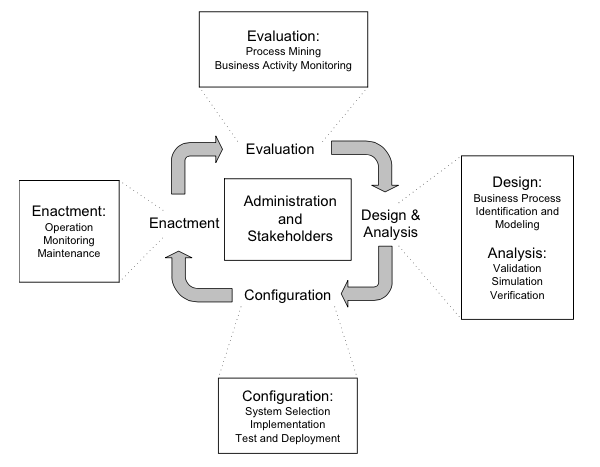
\includegraphics[width=1.0\textwidth]{obrazky/processLifecycle}
\caption{Business Process Lifecycle \cite{Weske2007}}
\label{fig:BusinessProcessLifecycle}
\end{figure}

Ve fázi \textit{Návrh a analýza} dochází ke sběru informací o procesech většinou formou pohovorů a dotazování zodpovědných pracovníků. Na základě takto nasbíraných informací je možné procesy identifikovat, popsat, potvrdit se zodpovědnými pracovníky a vytvořit jejich Business Process Modely.

Po návrhové fázi většinou následuje fáze \textit{Implementace}. Podnikový proces může být implementován například pouze \uv{slovně} pomocí souboru pravidel a opatření, které musí zodpovědní zaměstnanci dodržovat. Často je ale k realizaci podnikových procesů využíván specializovaný software. V takovém případě dochází k obohacení Business Process Modelu o specificky technické informace a také o doplnění interakcí pracovníků se softwarem.

Ve chvíli, kdy je dokončena implementace je možné přikročit k fázi \textit{Provádění}. Provádění konkrétní instance podnikového procesu je většinou spuštěno nějakou událostí (např. jiným procesem). V této chvíli systém BPMS aktivně kontroluje provádění procesu a upozorňuje zodpovědné pracovníky na případné problémy nebo požadavky na součinnost. V průběhu této fáze jsou také shromažďována cenná data, která prováděním procesu vzniknou. Tato data slouží jako vstup poslední vyhodnocovací fáze.

Fáze \textit{Vyhodnocení} využívá nasbíraná data, která jsou vyhodnocována a jsou v nich hledány příležitosti k optimalizaci procesu. Příkladem může být například, že některá část procesu trvá příliš dlouho z důvodu zpožďování dodávek materiálu. Na základě takové informace mohou manažeři přistoupit k úpravě procesu dodávání materiálů a dosáhnout tak časové úspory.

\subsection{Capability Maturity Model}
Capability Maturity Model (CMM) definuje pět stádií vyspělosti, kterými firmy a organizace procházejí při snaze porozumět vlastním podnikovým procesům. Jednotlivá stádia popisuje tabulka \ref{tab:cmm}.


\begin{table}[H]\centering
  \caption{Jednotlivá stádia vyspělosti v práci s podnikovými procesi dle modelu CMM \cite{Harmon2014}}
  \label{tab:cmm}
  \begin{tabular}{ | l | p{10cm} | }
    \hline
    \textbf{Stádium vyspělosti} & \textbf{Stav} \\ \hline\hline
    1. Initial & Procesy jsou vykonávány ad hoc bez jasně definovaných postupů. \newline Úspěch procesu závisí zejména na výkonu zodpovědných pracovníků. \\ \hline
    2. Repeatable & Základní techniky projektového řízení jsou již zavedeny pro sledování nákladů, plánování a definování funkcionalit. Je zaveden základní rámec, který umožňuje opakovat předchozí úspěšné provedení nějakého úkonu.  \\ \hline
    3. Defined & V této fázi je proces již dokumentován a standardy pro jeho provádění jsou definovány. \\ \hline
    4. Managed & Probíhá sběr výkonnostních měřítek pro vyhodnocování kvality provádění procesů. Procesy jsou prováděny pod dohledem.  \\ \hline
    5. Optimizing & Procesy jsou na základě nasbíraných dat a zpětné vazby neustále vylepšovány za účelem jejich zefektivnění.  \\
    \hline
  \end{tabular}
\end{table}

\subsection{Classification of Business Processes}
\subsection{Klíčové role při řížení podnikových procesů}


\section{Vývoj přístupů k řízení podnikových procesů}

\bibliographystyle{plain}
\bibliography{Bibliography}

\end{document}